%%%%%%%%%%%%%%%%%%%%%%%%%%%%%%%%%%%%%%%%%
% Beamer Presentation
% LaTeX Template
% Version 2.0 (March 8, 2022)
%
% This template originates from:
% https://www.LaTeXTemplates.com
%
% Author:
% Vel (vel@latextemplates.com)
%
% License:
% CC BY-NC-SA 4.0 (https://creativecommons.org/licenses/by-nc-sa/4.0/)
%
%%%%%%%%%%%%%%%%%%%%%%%%%%%%%%%%%%%%%%%%%

%----------------------------------------------------------------------------------------
%	PACKAGES AND OTHER DOCUMENT CONFIGURATIONS
%----------------------------------------------------------------------------------------

\documentclass[
	11pt, % Set the default font size, options include: 8pt, 9pt, 10pt, 11pt, 12pt, 14pt, 17pt, 20pt
	%t, % Uncomment to vertically align all slide content to the top of the slide, rather than the default centered
	aspectratio=169, % Uncomment to set the aspect ratio to a 16:9 ratio which matches the aspect ratio of 1080p and 4K screens and projectors
]{beamer}

\graphicspath{{Images/}{./}} % Specifies where to look for included images (trailing slash required)

\usepackage{booktabs} % Allows the use of \toprule, \midrule and \bottomrule for better rules in tables

\usepackage{tikz}
\usepackage{colortbl}

\usetikzlibrary{shapes,arrows,positioning}

\usepackage{graphicx}
%----------------------------------------------------------------------------------------
%	SELECT LAYOUT THEME
%----------------------------------------------------------------------------------------

% Beamer comes with a number of default layout themes which change the colors and layouts of slides. Below is a list of all themes available, uncomment each in turn to see what they look like.

%\usetheme{default}
%\usetheme{AnnArbor}
%\usetheme{Antibes}
%\usetheme{Bergen}
%\usetheme{Berkeley}
%\usetheme{Berlin}
%\usetheme{Boadilla}
%\usetheme{CambridgeUS}
%\usetheme{Copenhagen}
%\usetheme{Darmstadt}
%\usetheme{Dresden}
%\usetheme{Frankfurt}
%\usetheme{Goettingen}
%\usetheme{Hannover}
%\usetheme{Ilmenau}
%\usetheme{JuanLesPins}
%\usetheme{Luebeck}
\usetheme{Madrid}
%\usetheme{Malmoe}
%\usetheme{Marburg}
%\usetheme{Montpellier}
%\usetheme{PaloAlto}
%\usetheme{Pittsburgh}
%\usetheme{Rochester}
%\usetheme{Singapore}
%\usetheme{Szeged}
%\usetheme{Warsaw}

%----------------------------------------------------------------------------------------
%	SELECT COLOR THEME
%----------------------------------------------------------------------------------------

% Beamer comes with a number of color themes that can be applied to any layout theme to change its colors. Uncomment each of these in turn to see how they change the colors of your selected layout theme.

%\usecolortheme{albatross}
%\usecolortheme{beaver}
%\usecolortheme{beetle}
%\usecolortheme{crane}
%\usecolortheme{dolphin}
%\usecolortheme{dove}
%\usecolortheme{fly}
%\usecolortheme{lily}
%\usecolortheme{monarca}
%\usecolortheme{seagull}
%\usecolortheme{seahorse}
%\usecolortheme{spruce}
%\usecolortheme{whale}
%\usecolortheme{wolverine}

%----------------------------------------------------------------------------------------
%	SELECT FONT THEME & FONTS
%----------------------------------------------------------------------------------------

% Beamer comes with several font themes to easily change the fonts used in various parts of the presentation. Review the comments beside each one to decide if you would like to use it. Note that additional options can be specified for several of these font themes, consult the beamer documentation for more information.

\usefonttheme{default} % Typeset using the default sans serif font
%\usefonttheme{serif} % Typeset using the default serif font (make sure a sans font isn't being set as the default font if you use this option!)
%\usefonttheme{structurebold} % Typeset important structure text (titles, headlines, footlines, sidebar, etc) in bold
%\usefonttheme{structureitalicserif} % Typeset important structure text (titles, headlines, footlines, sidebar, etc) in italic serif
%\usefonttheme{structuresmallcapsserif} % Typeset important structure text (titles, headlines, footlines, sidebar, etc) in small caps serif

%------------------------------------------------

%\usepackage{mathptmx} % Use the Times font for serif text
\usepackage{palatino} % Use the Palatino font for serif text

%\usepackage{helvet} % Use the Helvetica font for sans serif text
\usepackage[default]{opensans} % Use the Open Sans font for sans serif text
%\usepackage[default]{FiraSans} % Use the Fira Sans font for sans serif text
%\usepackage[default]{lato} % Use the Lato font for sans serif text

%----------------------------------------------------------------------------------------
%	SUPRESSING AUX FILE DIRECTORY
%----------------------------------------------------------------------------------------

%----------------------------------------------------------------------------------------
%	SELECT INNER THEME
%----------------------------------------------------------------------------------------

% Inner themes change the styling of internal slide elements, for example: bullet points, blocks, bibliography entries, title pages, theorems, etc. Uncomment each theme in turn to see what changes it makes to your presentation.

%\useinnertheme{default}
\useinnertheme{circles}
%\useinnertheme{rectangles}
%\useinnertheme{rounded}
%\useinnertheme{inmargin}

%----------------------------------------------------------------------------------------
%	SELECT OUTER THEME
%----------------------------------------------------------------------------------------

% Outer themes change the overall layout of slides, such as: header and footer lines, sidebars and slide titles. Uncomment each theme in turn to see what changes it makes to your presentation.

%\useoutertheme{default}
%\useoutertheme{infolines}
%\useoutertheme{miniframes}
%\useoutertheme{smoothbars}
%\useoutertheme{sidebar}
%\useoutertheme{split}
%\useoutertheme{shadow}
%\useoutertheme{tree}
%\useoutertheme{smoothtree}

%\setbeamertemplate{footline} % Uncomment this line to remove the footer line in all slides
%\setbeamertemplate{footline}[page number] % Uncomment this line to replace the footer line in all slides with a simple slide count

%\setbeamertemplate{navigation symbols}{} % Uncomment this line to remove the navigation symbols from the bottom of all slides

%----------------------------------------------------------------------------------------
%	BILIOGRAPHY PACKAGE
%----------------------------------------------------------------------------------------

\usepackage[backend=biber,bibencoding=utf8,style=authoryear]{biblatex}

%----------------------------------------------------------------------------------------
%	Roadmap
%----------------------------------------------------------------------------------------


\setbeamerfont{myTOC}{series=\bfseries, size=\Large}
\AtBeginSection[]{
        \frame{
            \frametitle{Roadmap}
            \tableofcontents[current]   
        }
    }

%----------------------------------------------------------------------------------------
%	Configuration of Footer
%----------------------------------------------------------------------------------------

\setbeamertemplate{navigation symbols}{} 

\makeatletter


\setbeamertemplate{footline}{%
  \raisebox{5pt}{\makebox[\paperwidth]{\hfill\makebox[10pt]{\scriptsize\insertframenumber}}}}

%----------------------------------------------------------------------------------------
%----------------------------------------------------------------------------------------
%	PRESENTATION INFORMATION
%----------------------------------------------------------------------------------------

% Title --------------------------------------------
\title{LLMs: Applications to Economics Research}
\subtitle{Honors Thesis Class}
\date{\today}
\author{Nathan Williams}
\begin{document}
%---------------------------------------------------
\begin{frame}
\maketitle
\end{frame}
%---------------------------------------------------
\section{Introduction}
%---------------------------------------------------
\begin{frame}{Questions}
    \begin{enumerate}
        \setlength{\itemsep}{20pt}
        \item How many of you have used ChatGPT or another LLM?
        \item How many of your professors have talked about it?
        \item Have you had good experiences? Bad experiences?
    \end{enumerate}
\end{frame}
%---------------------------------------------------
\begin{frame}{Why are we talking about AI and Research?}
    The proliferation of AI applications and Large Language Models for academic research has increased drastically in the schools.
    \begin{figure}
        \centering
        
\includegraphics{News Screeenshot 1.png}
        \label{News Article}
    \end{figure}
\end{frame}
%-------------------------------------------------
\begin{frame}{Professors are adapting too!}
    \begin{figure}
        \centering
        \includegraphics[scale=.7]{AI_adoption.png}
        \label{Tweet}
    \end{figure}
\end{frame}
%-------------------------------------------------
\begin{frame}{Artificial Intelligence Platforms}
    The popularity of ChatGPT and OpenAI has led to the proliferation of many AI platforms
    \begin{itemize}
        \item Github Copilot
        \item StableLM
        \item Pythia
        \item BloombergGPT
    \end{itemize}
    \vspace{20pt}
    This space is growing so quickly that there will likely be one announced over the course of this presentation. \textbf{
        We will focus on ChatGPT and Github Copilot.}
\end{frame}
%------------------------------------------------
\begin{frame}{Using AI in Research}
    Using generated work in research can be very dangerous for the following reasons:
    \vspace{20pt}
    \begin{itemize}
        \item Incorrect Information
        \item Plagiarism
    \end{itemize}
    \vspace{20pt}
    The goal of this talk is to minimize the risks of either of these issues arising. 
\end{frame}
%----------------------------------------------
\begin{frame}{Is this talk anti-LLM?}
    \begin{center}
        \textbf{No!} I use it in my own research! (But I use it with caution!)
    \end{center}
\end{frame}
%-----------------------------------------------
\section{General Rules of Thumb}
%-----------------------------------------------
\begin{frame}{General Rule of Thumb}\label{Rule of Thumb}
    LLMs tend to do worse at generating original material, as they tend to make things up if not properly prompted.
    \bigbreak 
    \begin{block}{Rule of Thumb}
        Avoid having an LLM generate its own work, use it to enhance your already existing work
    \end{block}
\end{frame}
%-----------------------------------------------
\begin{frame}{Construction of Queries}
    Every time a query is constructed, think of choosing a set of additional information such that the probability of a correct answer is maximized. There are a few key aspects that consistently improve the outputs of LLMs. 
    \begin{itemize}
        \setlength{\itemsep}{20pt}
        \item Writing clear text
        \item Prompt Structure
    \end{itemize}
\end{frame}
%----------------------------------------------
\begin{frame}{Basic Prompt Structure (\href{https://www.promptingguide.ai/introduction/basics}{Source})}\label{Prompt Structure}
    A well-structured prompt can have up to 4 key elements. These are not all needed but can be valuable in answering more complicated questions. 
    \begin{itemize}
        \setlength{\itemsep}{20pt}
        \item Instruction
        \item Context
        \item Input Data
        \item Output Data
    \end{itemize}
\end{frame}
%-----------------------------------------------
\begin{frame}{Some Other Key Prompt Approaches (\href{https://www.promptingguide.ai/introduction/basics}{Source})}
    Many of the standard rules of thumb for Google searches often apply here:
    \begin{itemize}
        \setlength{\itemsep}{20pt}
        \item Specificity
        \item Start Smaller
        \item Avoid Impreciseness
    \end{itemize}
\end{frame}
%-----------------------------------------------
\section{Coding}
%-----------------------------------------------
\begin{frame}{Coding in LLMs}
    The largest efficiency gain for researchers comes from LLM's coding ability. 
    \begin{itemize}
        \setlength{\itemsep}{20pt}
        \item \textcolor{red}{Writing Code}
        \item Interpreting Errors
        \item Streamlining Speed
    \end{itemize}
\end{frame}
%-----------------------------------------------

%-----------------------------------------------
\begin{frame}{LLMs are not equally helpful}
    \begin{figure}
        \centering
        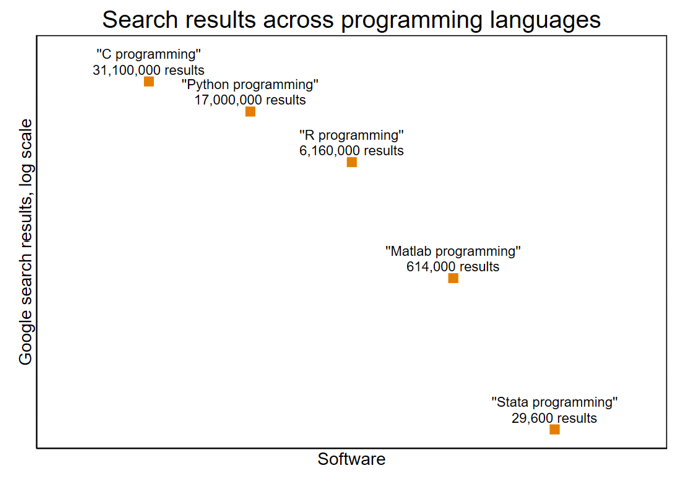
\includegraphics{Availability of Results on Internet.png}
    \end{figure}
\end{frame}
%-----------------------------------------------
\begin{frame}{Interpreting Errors}
    One of the most powerful tools LLMs can be used for is interpreting errors. Simply copy and paste your error into the interface window.

    \vspace{20pt} 
    This is not a substitute to StackOverflow, but rather a compliment.
\end{frame}
%-----------------------------------------------
\begin{frame}{Prompt Strategy - Interpreting and Fixing Errors}
    A better way to interpret errors can be borrowed from the \alert{prompt engineering} literature:
    \begin{enumerate}
        \setlength{\itemsep}{20pt}
        \item Set up the \hyperlink{Prompt Structure}{prompting environment}
        \item Include both your code and your error
        \item Ask the LLM to explain the error in the context of your code in the \alert{Output Data} section
    \end{enumerate}
\end{frame}
%-----------------------------------------------
\begin{frame}{Streamlining Speed}
    In every subfield of economics, there exists simulations that can take a very long time (days to weeks). Small coding optimizations can take a project that takes weeks to simulate and move it to days. 
    \vspace{15pt}
    \begin{itemize}
        \setlength{\itemsep}{20pt}
        \item Microeconomics (Bootstrapping)
        \item Macroeconomics (Model Estimation)
        \item Econometrics (Bootstrapping)
    \end{itemize}
    
\end{frame}
%-----------------------------------------------
\begin{frame}{Prompt Strategy - Speeding Up Code}
    \begin{enumerate}
        \setlength{\itemsep}{20pt}
        \item Set up the \hyperlink{Prompt Structure}{prompting environment}
        \item Include your code in the \alert{Context} section
        \item Ask the LLM to find ways to optimize your code
    \end{enumerate}
\end{frame}
%-----------------------------------------------
\begin{frame}{Generating New Code}
    Per the \hyperlink{Rule of Thumb}{Rule of Thumb Slide}, it is a good idea to avoid an LLM generating all code for a few key reasons:
    \begin{itemize}
        \setlength{\itemsep}{20pt}
        \item The LLM may hallucinate packages or commands, especially as the program has less active resources on the internet (read: \alert{Stata}) 
        \item The prompt and structure must be very specific
        \item You still have to know what the code does! 
        \item Certain people may construe this as academic dishonesty
    \end{itemize}
    \alert{It is in your best interest not to do this.}
\end{frame}
%-----------------------------------------------
\begin{frame}{Demo Time!}
    \begin{enumerate}
        \setlength{\itemsep}{20pt}
        \item Find some code that you have written that you \textbf{understand}
        \item Ask ChatGPT how to do write it using the prompting structure discussed
        \item Paste your code into ChatGPT and ask it to interpret it
        \item How does it do?
    \end{enumerate}
\end{frame}
%-----------------------------------------------
\section{Writing}
%-----------------------------------------------
\begin{frame}{LLMs are editors, not writers}
    Unlike with code, using an LLM to write for you is widely considered \alert{academic dishonesty} and you should not do it ever!

    \vspace{20pt}
    However, there are some uses for ChatGPT with writing that are both largely permissible and can serve to help you in your own writing.
\end{frame}
%----------------------------------------------
\begin{frame}{Writer's Voice}
    \begin{figure}
        \centering
        \includegraphics[scale=.5]{moura_tweet.png}
        \label{Writer's Voice}
    \end{figure}
\end{frame}
%----------------------------------------------
\begin{frame}{Why use an LLM to edit work?}
    One of the most popular strategies of editing is reading your work aloud to a friend (or yourself, no judgement). 
    This helps discern the quirks of your \alert{voice} that you otherwise might not see.

    \bigbreak
    If you don't have friends, ChatGPT and other LLMs can serve this purpose.
\end{frame}
%----------------------------------------------
\begin{frame}{Prompt Strategy - Editing Documents}
    \begin{itemize}
        \item Set up the \alert{prompting environment}, make sure the LLM knows it is an editor and not a writer
        \item Paste a section of the document that you would like to be edited and ask ChatGPT to edit it
    \end{itemize}
\end{frame}
%----------------------------------------------
\begin{frame}
    \begin{center}
        \huge{Demo Time!}
    \end{center}
    \begin{enumerate}
        \item Find some writing that you have done for another class
        \item Ask ChatGPT to edit it
        \item How does it do?
    \end{enumerate}
\end{frame}
%----------------------------------------------
\section{Conclusion}
%----------------------------------------------
\begin{frame}{LLMs and ChatGPT}
    Both are powerful, but dangerous tools in the research process. Please use caution when using. 
    \bigbreak
    
    If you have any questions, come see Hanna or Nathan and we will help you :)
\end{frame}
%----------------------------------------------
\end{document}